\chapter{Reduced precision}
\label{ch:reduced-precision}
\HL{Computing applications are usually developed to use the maximum precision (e.g., double precision).}
While this is necessary for specific fields (e.g., aerospace), results obtained at a lower
precision are acceptable in many contexts.
As~\cite{Cherubin2020-tt} depicts, numerous studies explored the use of lower
precision data types to perform computations.
It is an interesting strategy as it has the joint potential to reduce hardware
size, energy cost, and execution time.
In this chapter, we present (1) the problem definition of \textit{Reduced Precision},
(2) various data formats used to perform reduced precision,
(3) methods to implement reduced precision,
(4) the growth of quantization in Deep Learning,
and (5) the benefits, limitation, and open questions of reduced precision.

\section{Problem definition}
\label{sc:rp-problem-definiton}
The IEEE~754 standard defines two main floating-point formats: FP32 and FP64.
However, not all types of applications require that much precision.
For this reason, many efforts were put into creating new data formats with lower precision (discussed in Section~\ref{sc:rp-data-format}).
The idea behind reduced precision is to represent numbers in a data format with
lower bit width, i.e., lower exponent or mantissa.
Similarly, mixed-precision is a concept that uses data formats of different precision within a program, allowing for better precision tunning.
The logic complexity of floating points is approximately proportional to the square of the bit width~\cite{Chen2018-an}.
Therefore, lowering the number of bits in a data format also reduces the die size
of a chip and, consequently, the energy cost and computation time for arithmetic operations.

The work in~\cite{Cherubin2020-tt} surveys a range of tools in the fields of reduced precision.
That same study defines five challenges that remain to be addressed for reduced precision:
\begin{itemize}
	\item[1.] Identify the code sections where applying reduced precision is beneficial;
	\item[2.] Determine the data type to use based on the application and architecture;
	\item[3.] Estimate, quantify bounds, and manage the numerical error introduced by applying reduced precision to an application;
	\item[4.] Measure the overhead from type casting between different data types;
	\item[5.] Develop a tool that benefits many applications and platforms.
\end{itemize}
The authors of this study claim that reduced precision will not be sustainable
in commercial or open-source applications without solving those limitations and
will mostly remain an academic subject.
Moreover, the current lack of tools to perform code conversion makes reduced precision
a significant development effort.
Overall, developing a tool that can be applied to multiple use cases and
architectures is an open issue~\cite{Cherubin2020-tt}.

\section{Data formats for reduced precision}
\label{sc:rp-data-format}
Although Chapter~\ref{ch:background} focused primarily on the IEEE~754 Binary data format, many other data formats exist.
This section introduces other data types used in reduced precision studies.

Common Deep Learning frameworks such as Tensorflow~\cite{tensorflow2015-whitepaper} and Pytorch~\cite{PyTorch_2019} support mixed-precision through their API.
Both frameworks support the classical IEEE float32 and float16 with the addition to the \textit{bfloat16} introduced by Google Brain~\cite{bfloat16}.
As shown in Figure~\ref{fig:bfloat16}, the bfloat16 is a 16-bit floating-point format that uses
the same number of bits as the IEEE float32 for its exponent while having shorter bit width for its mantissa.
\begin{figure}[b]
	\centering
	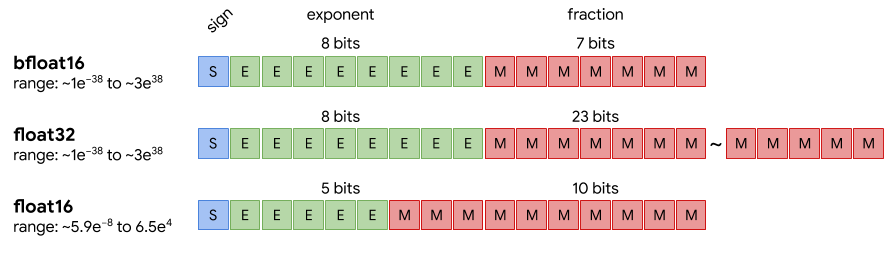
\includegraphics[width=\textwidth]{bfloat16.png}
	\caption{Representation of the bfloat16 format. (Taken from~\cite{bfloat16})}
	\label{fig:bfloat16}
\end{figure}
With the same exponent length as float32, bfloat16 allows for quick data type
conversions by dropping or adding the extra bits between float32 and bfloat16.
Moreover, with a smaller mantissa size, hardware chips for the bfloat16 multiplier
are about half the size of float16 ones and around eight times smaller than for float32~\cite{bfloat16}.
Additionally, since Neural Networks (NNs) are far more sensitive to the exponent range than the mantissa,
the bfloat16 performs well as it keeps the exponent range from float32.

Outside of standard Deep Learning frameworks, various data types were
studied to reduce the precision of machine learning models.
The work from~\cite{Johnson2018-up} evaluates a new \textit{posit tapered} data
format which combines ideas from the posit~\cite{Gustafson2017-wo} format and the log number system~\cite{Kingsbury1971-kx}.
Various other studies use different custom floating-point formats with reduced
exponent and mantissa size~\cite{Lesser2011-mn, Chen2018-an, Vicuna2021-mw, Wang2018-oo}.
The authors in~\cite{Carmichael2019-nu} designed three FPGAs for low-precision fixed-point, floating-point, and posit.

\section{Implementing reduced precision}
To remain efficient, consumer hardware only supports a limited set of data formats; for example, IEEE~754.
In addition, custom data formats often require specialized hardware, software implementation, or simulation. 

Implementing a new format can be tricky, with commodity hardware only supporting the most popular data formats.
A straightforward way to achieve this is to design custom specialized hardware capable of executing the new format.
The authors in~\cite{Carmichael2019-nu} designed three different FPGAs to support low-precision floats, fixed points, and posits.
Another study~\cite{Johnson2018-up} designed a \SI{28}{\nano\meter} ASIC to implement an 8-bit Exact Multiply-Accumulator (EMAC).
On the one hand, the main advantage of designing specialized hardware is efficiency.
Indeed FPGAs and ASICs designed for single tasks can be optimized much more than general-purpose hardware.
For example, major hardware manufacturers such as Nvidia, Google, and Intel
design specialized hardware for frequent Deep Learning tasks (GEMMs) with their
recent GPU architectures and TPUs~\cite{tpu,intel-BF16-2018}.
On the other hand, creating new hardware is costly in time and material.
This is especially true when performing a study that evaluates a range of different data formats.

Since hardware implementations can be challenging, some research investigated
software solutions to implement reduced precision.
In~\cite{Anderson2016-yn}, the authors proposed a new data format, \textit{flyte},
with a mantissa that differs in 8-bits increment from the traditional IEEE~754
standard while keeping the exponent the same.
This allows native instructions to read data with power-of-two bit width.
The authors suggest a packing and shuffling method to prevent cache miss due to misalignment by reorganizing the flyte in the vector registers.
However, some issues with misalignment for some flyte formats resulted in a lower performance gain.
Overall, their technique significantly reduces cache misses for \textit{BLAS} Level 2 and 3; as many as $4.5\times$ less than double precision.
The authors in~\cite{Zucker1994-rg} propose an algebraic method to pack multiple
low-precision operations into a single high-register operation.
This method showed a performance improvement of 8.7\%, 13.6\%, and 16.2\% when packing
2, 4, and 8 numbers, respectively.
Unfortunately, this technique can only be applied to a few algebraic operations.
On the one hand, software implementations are less efficient than specialized hardware
since they suffer from substantial overhead costs.
Often, implementing software solutions requires high manual efforts, whether to
perform code conversion or design a new data format.
On the other hand, software design can be more portable across architecture than specialized hardware.

As an alternative to hardware or software implementation, a common approach to
prototype or study new data formats is through simulation.
The work in~\cite{Chatelain2019-fu} explores reduced precision to lower the communication costs of iterative methods.
They use the VPREC backend in Verificarlo to simulate reduced precision combined
with a heuristic to determine a minimum precision for the different iterations.
They consider both temporal and spatial changes in the precision of applications.
Other studies~\cite{Higham2019-yd,Zhang2019-xv} propose simulation methods for reduced
precision on single operations and kernels.
The work in~\cite{Higham2019-yd} implemented a reduced precision library in MATLAB, and
the work in~\cite{Zhang2019-xv} developed a high-level framework on top of PyTorch to use
reduced precision techniques.
The main benefits of simulating reduced precision are the low implementation cost and new hardware not needing to be designed.
This often allows exploring a large number of data formats with fewer efforts.
Unfortunately, while simulations are great for accuracy evaluation, it is still challenging to simulate performance due to the complexity of modern systems.
Moreover, simulating reduced precision comes at a substantial overhead cost.
Therefore, it is required to implement a hardware or software implementation later to achieve performance.

\section{Quantization in Machine Learning}
In recent years, machine learning, and more specifically Deep Neural Networks (DNNs),
have seen a rise in popularity due to their ability to solve challenging problems.
However, the complexity of DNN models comes with a high usage of computing resources.
With the enormous datasets required to train these models, compute and data communication time is usually a bottleneck.
This motivated multiple studies \cite{Johnson2018-up,Wang2018-oo,Lesser2011-mn,Chen2018-an,Judd2015-kw,Vicuna2021-mw}
to explore the possibility of reducing the precision of the data format used to train those models.
This section explores the quantization methods developed in the Deep Learning domain to reduce models' computing and data communication.

The authors from multiple studies explored the effects of quantization for SVM classification
and found it possible to use minimal precision without accuracy loss.
In~\cite{Lesser2011-mn}, the authors investigate the impacts of reducing precision for SVM
classification and estimate the minimal precision required to achieve classification
without loss of accuracy. They performed three experiments:
(1) adding noise to parameters,
(2) using MPFR, simulating reduced mantissa precision from 53 to 4 bits,
and (3) combining the experiment (1) and (2) concurrently.
By comparing the effects of quantization with and without rounding, it is possible to isolate better
the impact of rounding due to reduced precision.
The authors benchmark their experiments on three datasets: SONAR, IRIS, and MUSK.
They use the double precision results as a reference for the classification error.
The results show that lowering the precision up to 15 bits does not affect the accuracy
for classification.
Further understanding the bounds for reducing the precision would allow to automatically
adjust the precision for classification, which would be an effort towards addressing the third
challenge from Section~\ref{sc:rp-problem-definiton}.

With the increasing complexity of  DNNs, it becomes difficult to train the models with
techniques to improve performance, such as data sampling or model parallelism.
It is also problematic to integrate those models into embedded systems due to resource limitations.
While many studies found that CNNs are resilient to accuracy loss when using reduced precision,
few of them attempted to vary the precision used at each layer.
The authors in~\cite{Judd2015-kw} show that the precision required in different layers and networks differ significantly.
Moreover, they suggest a method to select the appropriate precision of each layer while
keeping accuracy within a determined boundary.
Their model converts floating points to the appropriate representation and then back to single-precision after processing a layer.
To evaluate their method, the authors benchmark their reduced precision model on five popular CNNs.
Through their experiments, they reduce the precision of both the model's weights and the output of each layer.
Their first experiment reduced the precision of all layers simultaneously in the range of 12 to 1 bits.
The results show that only 21 bits would be required to store both the weight and output data of a layer.
Next, the authors reduced the precision of individual layers to obtain the importance of precision for each layer.
From the results, we observe that the precision required by each layer varies significantly.
The authors also calculate an estimated data communication for the networks.
Finally, they also propose a method to find the minimal precision per layer while preserving accuracy:
\begin{itemize}
	\item[1.] Set the layers to an initial uniform precision with less than $0.1\%$ error.
	\item[2.] Create a collection of deltas by reducing the precision of parameters and layer output by 1 bit for each layer.
	\item[3.] Use the configuration with the best accuracy for the next iteration.
\end{itemize}
To find the best mixed-precision, although potentially sub-optimal, the authors use a Pareto
frontier between the amount of data transfer and the accuracy for different configurations of bit precision.
Although sub-optimal, this heuristic resulted in an average decrease of $74\%$ of data traffic
while preserving accuracy within $1\%$ of tolerance.
This work shows the potential of using various precision sizes for different layers of CNNs.
Furthermore, it motivates further efforts to study strategies in further exploiting reduced precision to reduce memory usage and compute time.

Linear algebra operations are critical components in most DNNs models such as
the multiply-accumulate (MAC) operation ($\sum_{i}a_{i}b_{i}$).
The authors in~\cite{Johnson2018-up} describe \textit{ELMA}, a new method to compute MAC using a combination of the logarithmic
number system~(LNS), \textit{Kulisch accumulator}~(EMA), and the posit data format~\cite{Gustafson2017-wo}.
The authors evaluate the accuracy using an FPGA implementation of the ResNet-50~ImageNet model.
Moreover, the new ELMA implementation is compared in the area~($\SI{}{\micro\metre}^2$)
and power~(\SI{}{\micro\watt}) using a \SI{28}{\milli\metre} ASIC library.
The results show that the proposed ELMA operator reduces the power usage on
multiplications by \SI{90.9}{\micro\watt} but increases it for additions by \SI{68.3}{\micro\watt}.
Overall, the net power usage is lower than in previous methods suggesting that
further efforts to reduce floating-point efficiency could bring substantial benefits.

Without a doubt, DNNs emerged as a powerful tool to solve problems.
However, to achieve high accuracy, DNNs require a tremendous amount of resources;
with models reaching 100s of \SI{}{\mega\byte}s, and computation on large datasets can span multiple days/weeks.
In~\cite{Chen2018-an}, the authors explore approximate computing to reduce both 
computation and data communication of DNNs, while preserving accurate results.
The authors quantize the weight and activation of the model from 16 to 2 bits.
Then, the authors benchmark the reduced precision model on four popular DNNs to evaluate its accuracy.
They find that at 4 bits, the accuracy remains within $<1\%$ of the reference
full-precision model while improving performance by $4.5\times$.
When reducing the precision of the models to 2 bits, the authors achieve a $14\times$
improvement in normalized chip density, resulting in lower energy consumption.
Overall, the results from this paper show promising benefits to further studying
reduced precision strategies as it jointly reduces hardware and energy cost and
computing and data communication time. 

Numerous approximate computing methods have been studied for deep learning to
reduce computation and data communication time and energy cost.
The energy efficiency of hardware approximately increases quadratically with the reduction in bit precision~\cite{Wang2018-oo}.
With current hardware implementing 16 bits of precision, we can see performance improvements of $\ge 4\times$ compared to 32 bits.
Studies showed that the computation steps for DNNs inference could be reduced to as low as 2-4 bits
while remaining accurate, and even precision of 1-2 bits for weights and activations.
However, an empirical study found that a precision of 16 bits was required during
DNNs training to preserve accuracy.
When trying to reduce the precision further, DNNs often start to see significant
accuracy degradation, issues with convergence, and an impact on overall accuracy.
The authors in~\cite{Wang2018-oo} suggest using \textit{FP8} combined with 
\textit{chunk-based computations} and \textit{stochastic rounding} to further reduce
the bit precision compared to state-of-the-art methods while maintaining accuracy.
They evaluate their methods on a collection of 6 NNs models across multiple datasets.
The results show that their implementation using both FP8 and FP16 is equivalent
in accuracy to FP16 and FP32 while performing $2-4\times$ faster.
Moreover, the authors found that keeping a higher accuracy (FP16) on the first layer~(input data)
and the last layer was critical in training their FP8 models successfully.
This work shows that effort in reducing floating-point precision in deep learning
can increase performance significantly while keeping accuracy equivalent.

While machine learning models are a great tool to solve problems, they can be challenging
to implement on embedded systems due to their large memory requirement.
Mondrian Forest, an online classifying algorithm, is typically too memory-intensive
for embedded devices; therefore, using reduced precision could enable its use.
The authors in~\cite{Vicuna2021-mw} explore reduced precision techniques on Mondrian Forests
to reduce their memory usage.
They study the model parameters, numerical precision, and memory consumption together
due to their interdependence.
Using VPREC, the authors simulated reducing the bit precision $p$ from 52 to 1 bit.
Moreover, the exponent range is varied from 11 to 2 bits.
The model is instrumented both at a node level and for the whole model.
To evaluate their method, they use two publicly available datasest: Recofit, and Banos et al.
To quantify the model's performance with different memory constraints, the authors allocate three
different values of memory limit for the model: \SI{0.6}{\mega\byte}, \SI{1.2}{\mega\byte}, and \SI{3}{\mega\byte}.
Their results for node instrumentation show that for $p \ge 2$ the F1 scores remain with a standard deviation.
However, the F1 scores are significantly different for the complete instrumentation when $p \le 6$.
The observations on the F1 scores for $p > 2$ were not correlated to memory.
This suggests that using reduced precision with different memory allocations would yield similar results.
Given constant memory constraints, the authors found that reducing precision allows the
trees to grow deeper, potentially improving the classification performance.
Overall, the results show that Mondrian Forest can be implemented with an 8-bit floating-point
format without affecting the F1 scores significantly, which has the potential to
reduce memory footprint by roughly $1.8\times$ compared to double precision.

Although Section~\ref{sc:rp-data-format} discussed reduced and mixed precision
in popular deep learning frameworks like PyTorch and Tensorflow, the scope of
ultra-low precision (i.e., $\le 8$ bits) is still a topic limited to academia.
Further efforts are required to understand better the effects of reduced precision 
on different models and datasets; without it, the reach of ultra-low floating-point will remain restrained.
Furthermore, while the deep learning community has vastly explored reduced precision
techniques to the best of our knowledge, the topic remains unexplored in most other fields of application.

\section{Discussion}
\label{sc:reduced_precision_discussion}
In this chapter, multiple studies showed promising reduced precision approaches
to improve the performance of applications while preserving accuracy.
However, reduced precision comes with its caveats.
We will discuss the benefits and limitations of using reduced precision throughout this section.
Moreover, we will discuss open problems in the field of reduced precision.

By reducing the number of bits used to represent numbers, the memory footprint
of applications is directly reduced.
This has two main benefits: applications require fewer resources to execute, reducing the hardware cache miss, which increases performance.
Additionally, reducing the size of the data format allows specialized hardware
or software techniques to pipeline operations together.
With hardware complexity being approximately proportional to the square of the
number of bits~\cite{Chen2018-an}, reducing the data format can jointly increase
performance and reduce energy costs.
Furthermore, fusing multiple low-precision data format operations in a single register operation can lower computational costs. 
Lastly, reducing the size of input and output data would lower storage space requirements.

Using reduced precision requires substantial efforts for creating, evaluating, and implementing new data formats.
\HL{This is amplified by the current lack of understanding of the effects of applying
reduced precision to various applications and, in general, the precision required for a specific application.}
Even within a single application, varying the data can substantially modify the
precision required to preserve accurate results.
Finally, the conversion between data formats comes with an overhead cost.
Thus, attention must be paid to minimizing the amount of data format conversions
within an application when applying reduced precision.
Otherwise, the performance benefits from using reduced precision might be overtaken
by a high overhead cost in data conversion and result in an overall slowdown
in the performance of an application.
\HL{
	While hardware is an efficient way to implement reduced precision, it is also costly
	in time and material.
	On the opposite, software implementation is less efficient but tends to be more portable.
	Lastly, simulating reduced precision has a low implementation cost and does not
	require specialized hardware; however, it is limited to prototyping new data format and requires
	either a software or hardware implementation to improve performance.
}

To have a broader adoption of reduced precision, some critical limitations need to
be addressed, including but not limited to:
\begin{itemize}
	\item Determine the different sections of code that can take advantage of reduced precision
	      while considering both temporal and spatial variability of precision.
	\item Improve the heuristics for finding the minimal precision required for each code section.
	\item Estimate the performance gain from using reduced precision.
	\item Understand the effects of reduced precision when varying the data in an application.
	\item Automate the code conversion to simplify the usage of reduced precision.
\end{itemize}
To the best of our knowledge, these problems remain open challenges within reducing precision.
Therefore, further research will be needed to make progress in resolving these challenges.
